\section{Model 5: Network externalities}
In the earlier models, the experienced network effects only arose from their neighbours. I.e. when a node established a connection the change in utility were only dependent on fixed variables, and not dependent of the rest of the network. In many real world scenarios it is more realistic that a node will be strongly affected by the indirect connections to other nodes. Social relationships between nodes are good examples of such networks, where they offer benefits in terms of favors, information etc. 

We apply the results from the paper from Jackson and Wolinsky \cite{jackson1996strategic} and uses a network formation game found in \cite{jackson2005survey}, to study indirect networks effects in our model. 

The benefits a player receives in this game are calculated as follows. In addition to the benefit from the direct connection, a node will also benefit from "friends of the friend", and "friends of the friends of the friend" etc. This is achieved by letting the payoff be calculated relative to the distance between the nodes. $\beta$ is now dependent on the minimum number of hops to the node e.g. the benefit of a direct connection is $\beta$, the benefit of a friend of a friend is $\beta^2$ etc. We want the benefit to decrease with the distance, therefore we need the limitation: $0<\beta<1$. 
\begin{figure}[h]
\centering
  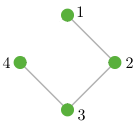
\includegraphics[width=0.3\linewidth]{../Figures/connectionGame.png}
  \caption{\label{fig:connectionGame} Four nodes interconnected with each other.}
\end{figure}
\subparagraph{Example:}Lets consider the network shown in \ref{fig:connectionGame}. Node 1 and node 4, in the network will receive a benefit of $\beta+\beta^{2}+\beta^{3}$ by being connected with node 2 and 3. $\beta^{2}+\beta^{3}$ represents the indirect benefits from node 3 and 4. Node 2 and 3 receives a benefit of $\beta+\beta+\beta^{2}$. For this network to make sense, it is important to also include some cost of having direct connections, or else the rational thing would be to establish a link with everyone. This is done as in earlier models, every node pay a cost for direct connections, but no cost for indirect connections. Thus the total payoff for a node is:

\begin{equation}
\sum_{j\neq i}^{} \beta_{ij}^{d(ij)} - \sum_{j:ij\in g}^{} {c}_{ij}, 
\label{eq:connecetionGame}
\end{equation}

where $d(ij)$ represents the shortest path between node $i $ and node $j $, and ${c}_{ij}$ represents node i's cost of establishing a link between the two nodes. To simplify the model we choose a symmetric connection process where $\beta$ and $c$ is set to a fixed global value. 

In the paper \cite{jackson1996strategic}, they analyze the networks with two differen approaches, one with focus on efficiency and the other on stability.  The optimal network is of course both efficient and stable, but as we shall see there are some conflicts between efficiency and stability. They showed that an efficient network is:
\begin{enumerate}
\item \textit{a complete graph $g^N$ if $c<\beta - \beta^2$,}
\item \textit{a star encompassing every node if $\beta - \beta^2 < c < \beta + \frac{(N-2)}{2}\beta^2$,}
\item \textit{an empty network(no links) if $\beta + \frac{(N-2)}{2}\beta^2 < c$.}
\end{enumerate}

The most efficient structure is a star structure which encompasses every node. A star structure have the characteristics of minimizing the average path length and uses the minimum number of links($N-1$) required for including every node. 
This structure provides the highest overall payoff for the network, but this network is not necessarily stable.

When analyzing the stability of the network, by using the definition of pairwise stability, Jackson and Wolinsky found four different stability conditions:

\begin{enumerate}
\item \textit{a pairwise stable network consists of at most one (non-empty) component,}
\item \textit{if $c<\beta - \beta^2$, the unique pairwise stable network will be a complete graph $g^N$, }
\item \textit{if $\beta - \beta^2 <c < \beta $, a star encompassing every node will be pairwise stable, although not necessarily the unique pairwise stable graph,}
\item \textit{if $\beta < c$ , any pairwise stable network which is nonempty is such that each player has at least two links and is thus inefficient. }
\end{enumerate}
We see that the stability condition 2, is the same as the efficiency condition 1, and thus if this condition is fulfilled, the network is both stable and efficient. 
Condition 3 shows us why the efficient star network is not necessarily  stable. If $\beta \leq c <   \beta + \frac{(N-2)}{2}\beta^2$ then the efficient network will be a star, but it is not stable.

It should be noticed that it is more beneficial for a node to operate as a leaf node compared to being a center node, due to the cost of direct connections. In a star structure, a leaf node will only have to pay the cost of the link to the center node, and will benefit indirectly for each node connected to the center node. The center node will benefit from each new connection, however, the payoff will only be $\beta - c$ for each connection. 

\subsection{Insurance and connection game}
The findings about efficiency and stability are very useful for our model, because if one has knowledge of the different variables it is possible to determine how the network will evolve. Additionally, if you are able to control the variables, you can actually determine the resulting network structure.
From the papers, we know that there exists different boundaries on the link cost, and how the resulting stable and efficient network will be.
Our earlier models shows that the cost of establish a link is the insurance cost and/or the risk cost. From this we can show that if $\beta - \beta^2 <I_{l}<\beta \text{ and } r>\beta$ a star with only insured nodes, and no connections between non-insured nodes, are both a stable and an efficient network. If $\beta - \beta^2 <I_{l}+r<\beta \text{ and } \beta - \beta^2<I_{l} \text{ and } \beta - \beta^2<r $ the stable and efficient network is a star consisting of both insured and non-insured nodes. If $I_{l}<\beta-\beta^2$ all insured nodes will connect to every other insured node, and if $r<\beta-\beta^2$ all non-insured nodes will connect to every other non-insured node.
In addition if $r+I_{l}<\beta-\beta^2$ the resulting network will be a clique of both insured and non-insured nodes.
The insurer can thus determine the formation of the network by adjusting the cost parameters. 

\subsection{Homogenous symmetric connection game}
From this point and on, the game we will consider is a homogenous network setting where every node is considered to be insured.
This is done because it will simplify an otherwise very complex model. We are analyzing the resulting network structure, which is easier when only considering one homogenous cost for every node.
Lets look at an example, where the parameters are set to: $\beta=0.9, I_{l}=0.5$, the resulting network are shown in Figure \ref{fig:stablestar}.



\begin{figure}[h]
\centering
  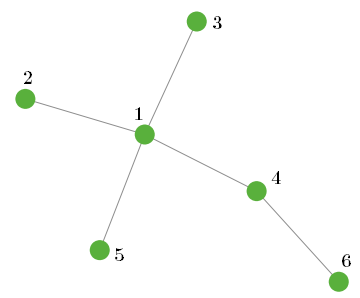
\includegraphics[width=0.5\linewidth]{../Figures/stability/Unefficientbutstablestar.png}
  \caption{\label{fig:stablestar} The resulting network after a simulation with the parameters $\beta=0.9, I_{l}=0.5$.}
\end{figure}
As we see this is not an efficient star, but the network is stable. The efficient network would be to delete the link $4,6$ and adding the link $1,6$. But since we only consider one link at a time this can not be done. To show this let $U_{i}$ denote the payoff of node $i$, the payoffs of the nodes are as described in Eq.(\ref{eq:payoffstablestar}).
\begin{eqnarray}
U_{1}=4\beta+\beta^2-4c\\
U_{2}=U_{3}=U_{5}=\beta+3\beta^2+\beta^3-c\\
U_{4}=2\beta+3\beta^2-2c\\
U_{6}=\beta+\beta^2+3\beta^3-c
\label{eq:payoffstablestar}
\end{eqnarray}
Node $6$ would benefit from adding the link $1,6$, but node 1 is not willing to do so because then he must pay an extra cost, and since $\beta^2>\beta-c$. Thus the network is stable but not efficient. 

From this we see that, even when the most efficient and the stable network is a star, we can not guarantee that the network formation game will end up in a star. This is because we only consider one link at a time, and not the whole network. 

\subparagraph{Star not possible with high \textit{n}.}
In the paper \cite{jackson2005survey} they came up with the following proposition:
Consider the symmetric connections model in the case where $\beta-\beta^2<c<\beta$. As the number of nodes grows, the probability that a stable state (under the process where each link has an equal probability of being identified) is reached with the efficient network structure of a star goes to zero. But if a network reaches the efficient star structure, it is also pairwise stable, and will remain a star. 
We confirmed this when running multiple simulations, when we used few nodes the resulting network often became a star, but as the number of nodes increased the network rarely became a star. 

However, the structure of the networks that evolve are very similar to a scale-free network. There are many nodes with low node degree, and few with a high node degree.
One example of this is shown in Figure \ref{fig:stablescalefree}, there are only ten nodes, but the network have the properties of a scale-free. Two nodes with degree of 4, and the rest have a degree of one or two.
\begin{figure}[h]
\centering
  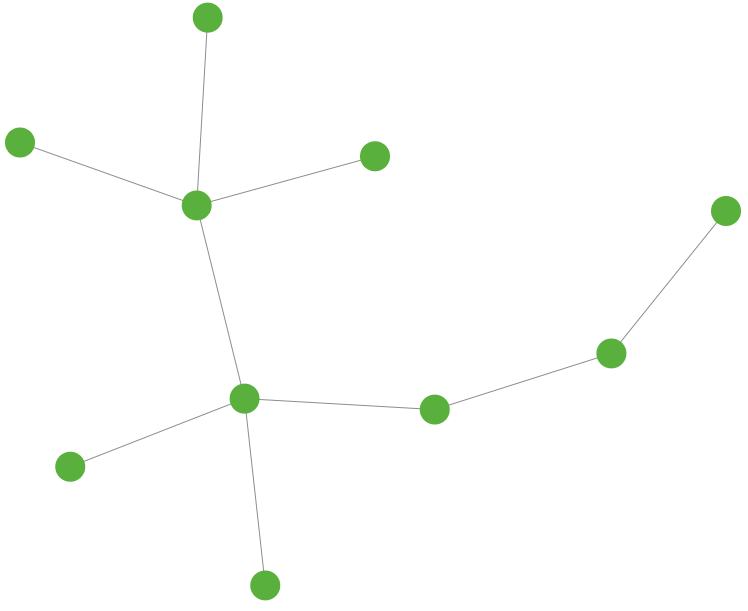
\includegraphics[width=0.6\linewidth]{../Figures/stability/Unefficientbutstabletwo.png}
  \caption{\label{fig:stablescalefree} The resulting network after a simulation with the parameters described earlier and 10 nodes.}
\end{figure}
\subparagraph{Bulk insurance.}
As noted before it is not preferable to be the center node, due to the cost of all the direct links. If we consider the model with bulk insurance discount, this would lower the extra cost for the center node significantly. This could be used to increase the probability of reaching a star formation. 

Using the discount formula from the previous model, we end up with Eq.(\ref{eq:discountstar}) to achieve a efficient and stable star topology. $i$ represents the node degree.
\begin{equation}
\beta-\beta^2<\frac{i_{l}}{i+1}< \beta
\label{eq:discountstar}
\end{equation}
An interesting property of the discount model is that the conditions for a efficient networks will change. Because
when the node degree increases, the insurance cost might reach the critical degree $g$, the best strategy for a node with degree $g$ or higher, is to connect to every node, as shown in Eq.(\ref{eq:criticaldiscount}). 
\begin{equation}
\frac{I_{l}}{g}<\beta-\beta^2
\label{eq:criticaldiscount}
\end{equation}
This is possible when $g<n$, where $n$-represents the number of nodes in the network.
The stability condition have changed for a node with a critical degree, the stable and efficient condition for this node is, as shown earlier, to have a direct connection to every other node. Thus if we have a star-topology both the leaf nodes and the center node are stable, and the center node has been compensated for its role in the network.

Since the networks formed are similar to scale-free networks, we can calculate the probability of a node having degree $g$, see Eq.(\ref{eq:probabilitydegree}). $\gamma$ is the power law parameter, as described in Chapter \ref{chp:graphTheory}.
\begin{equation}
P(g)=g^{-\gamma}
\label{eq:probabilitydegree}
\end{equation}
When a node $i$ reaches the critical degree $g$ its optimal strategy is to connect to every node, since the payoff generated from direct connections is larger than any indirect connection. In general nodes prefer to connect to nodes with high connectivity\footnote{A node with high degree implies a node with high connectivity.}, and will thus prefer to connect to this node compared to nodes with a degree lower than $g$. In this way nodes will connect to the node who have a degree greater or equal to $g$, and remove the links to their low-degree nodes which they can instead reach through the node with high connectivity.

Lets consider a case with $n-$nodes, and two of these nodes, $i$ and $j$, have an equal degree larger than $g$. The rest of the nodes has a degree of one or zero. If there exists a node with degree zero, it would prefer to be connected to $i$ or $j$, and so will $i$ and $j$, so this will eventually happen.
If a node connected to $i$ are considering connecting to $j$, or visa versa, it will do so because $j$ can offer a higher connectivity than $i$. Now $j$ has a higher degree than $i$, and thus every node would prefer to connect to $j$ over $i$. This will eventually result in a star formation, with $j$ as the center node.
From this we get the conjectures:
\begin{cnj}
If the critical degree ratio is low, i.e. the ratio between critical degree and number of nodes in the network, the resulting network will with high probability be a clique.
\label{prop:clique}
\end{cnj} 

\begin{cnj}
If the critical degree ratio is at a medium level, the resulting network will with high probability be a star. 
\label{prop:star}
\end{cnj}

\begin{cnj}
If the critical degree ratio is high, the resulting network will with high probability be a star-like/scale-free structure. 
\label{prop:scale-free}
\end{cnj}

A numerical example of the boundaries between the different structures, we found from our simulation (described in the next section) with 20 nodes that: 
As seen in Figure \ref{fig:PlotStar} a critical degree of 1-5 applies to conjecture \ref{prop:clique}, 6-12 applies to conjecture \ref{prop:star} and 13-20 applies to conjecture \ref{prop:scale-free}. 

\subsubsection{Results and findings}

To prove the conjectures above, we created a simulator. The rules of the simulator are as follows.
Every round two random nodes, not neighbors, are selected, and asked if they would want to establish a link. The link establishment is a symmetric decision, i.e. the link is established if it result in an increased payoff for both nodes. If the link is added, we check if either of the nodes would prefer to delete some of their already existing links, this decision is asymmetric. A link will be deleted if the node will achieve a higher payoff without it. Then we ask the rest of the nodes if they would like to delete any links. This procedure is repeated as long as there is possible to add new links. 
The payoff function of each node is as described earlier(see Eq.(\ref{eq:connecetionGame})), except that the cost is now dependent on the degree of the node. For the simulations to be realizable, we had to set the number of nodes to 20, or else the computational time was to high. For every critical degree, from three to nineteen, we ran 50 simulations, and noted the resulting network formation. We chose to start from critical degree equal three, since any number below would result in a clique, because it would be more beneficial to be directly connected to every node.  


We know that if Eq.(\ref{eq:discountstar}) is satisfied for all $i$, then the efficient and stable state is a star. But a more interesting scenario occurs when we have a graph where one or more of the nodes reaches the critical degree. -Will the final structure become a scale-free, a star or simply just unstructured? 
The results from the simulation can be seen in Figure \ref{fig:PlotStar}, \ref{fig:PlotClique} and \ref{fig:PlotStarIsj}. As we see from the figure \ref{fig:PlotStar}, the probability of the resulting network being a star, suddenly increases from zero to 42\% at critical degree five to six, and then jumps from 42 to 70-, 86-,96-, 98\% at critical degree six to nine. These results confirms our conjectures, and show that the discount can drastically increase the probability of the network ending up in a star. 

\begin{figure}
\centering
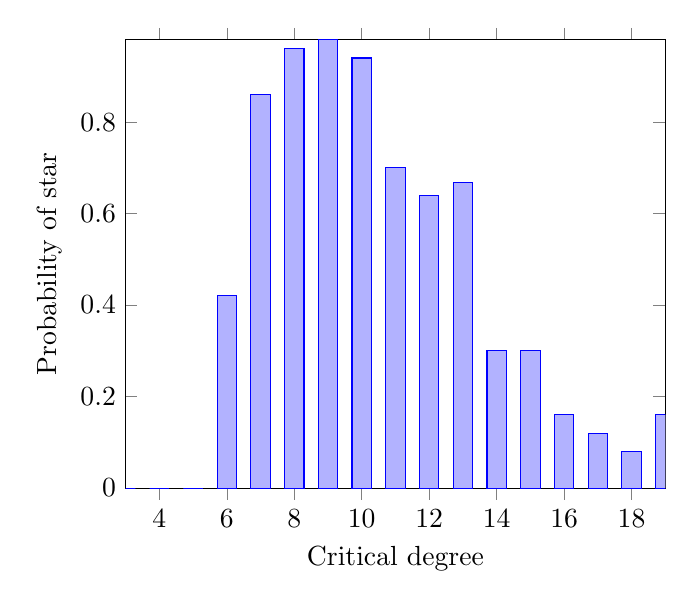
\begin{tikzpicture}
\begin{axis}[
x tick label style={
	/pgf/number format/1000 sep=},
	ylabel=Probability of star,
	xlabel=Critical degree,
enlargelimits=0.0,
legend style={at={(0.5,-0.15)},
anchor=north,legend columns=-1},
ybar,
bar width=7pt,
]
\addplot
coordinates {
(3,0.0) (4,0.0) (5,0.0) (6,0.42) (7,0.86) 
(8,0.96) (9,0.98) (10,0.94) (11,0.70) (12,0.64)
 (13,0.667) (14,0.3) (15,0.3) 
(16,0.16) (17,0.12) (18,0.08) (19,0.16) };
\end{axis}
\end{tikzpicture}
\caption{\label{fig:PlotStar} Shows the probability of the network ending up in a star given different critical degrees.}
\end{figure}

From Figure \ref{fig:PlotClique} we can observe that the opposite is happening, as the critical degree is increased, the probability of the resulting network being a clique, drastically decreases. As we can see with a critical degree of seven or higher, it is very unlikely that we end up with a clique. These findings also supports our conjectures.

\begin{figure}
\centering
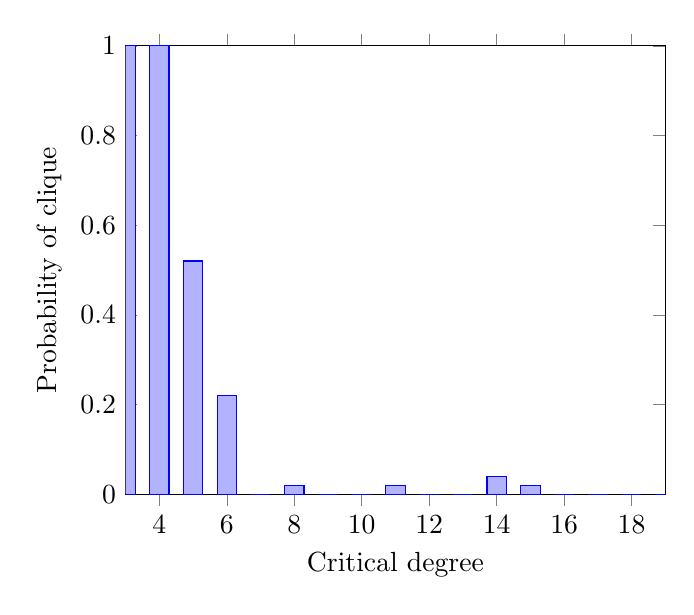
\begin{tikzpicture}
\begin{axis}[
x tick label style={
	/pgf/number format/1000 sep=},
	ylabel=Probability of clique,
	xlabel=Critical degree,
enlargelimits=0.0,
legend style={at={(0.5,-0.15)},
anchor=north,legend columns=-1},
ybar,
bar width=7pt,
]
\addplot
coordinates {
(3,1.0) (4,1.0) (5,0.52) (6,0.22) (7,0.0) 
(8,0.02) (9,0.0) (10,0.00) (11,0.02) (12,0.0)
 (13,0.0) (14,0.04) (15,0.02) 
(16,0.0) (17,0.0) (18,0.00) (19,0.0) };
\end{axis}
\end{tikzpicture}
\caption{\label{fig:PlotClique} Shows the probability of the network ending up in a clique, given different critical degrees.}
\end{figure}

An interesting comparison can be made between the emergence of a star versus a clique. In Figure \ref{fig:PlotStarVsClique}, shows a plot of the network resulting in a star and another plot of the probability the resulting network being a clique. As we can see, from a critical degree of five to seven, the resulting network structure, changes from almost certain ending up in a clique, to almost certain ending up in a star structure. The reason is as mentioned before that when the critical degree is low, the likelihood of many nodes reaching the critical degree is high. And none of these would like to delete any links. Hence we end up with a clique. The reason why we end up with star structures is because it is less likely that many nodes end up reaching the critical degree, hence it most of the nodes still prefer to rely on indirect links, but the ones who reach the critical degree prefer to connect to every one. Since the nodes with critical degree, have high connectivity, nodes will prefer to be connected with these, compared to other nodes. Nodes prefer to be connect to the ones with critical degree, the nodes with critical degree would like to connect to every one, and thus the structure evolves into a star, with the critical degree node in the center. 


\begin{figure}
\centering
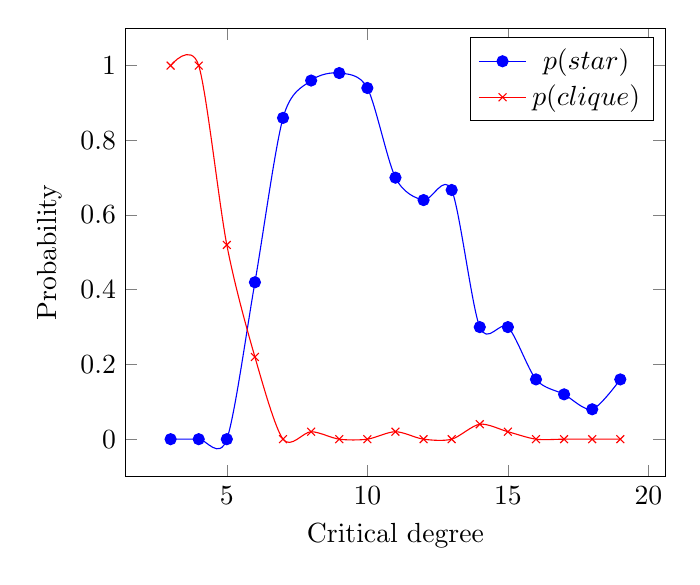
\begin{tikzpicture}
    \begin{axis}[
        xlabel=Critical degree,
        ylabel=Probability]
    \addplot[smooth,mark=*,blue] plot coordinates {
        (3,0.0) (4,0.0) (5,0.0) (6,0.42) (7,0.86) 
(8,0.96) (9,0.98) (10,0.94) (11,0.70) (12,0.64)
 (13,0.667) (14,0.3) (15,0.3) 
(16,0.16) (17,0.12) (18,0.08) (19,0.16)
    };
    \addlegendentry{$p(star)$}
    
    \addplot[smooth,color=red,mark=x]
        plot coordinates {
            (3,1.0) (4,1.0) (5,0.52) (6,0.22) (7,0.0) 
(8,0.02) (9,0.0) (10,0.00) (11,0.02) (12,0.0)
 (13,0.0) (14,0.04) (15,0.02) 
(16,0.0) (17,0.0) (18,0.00) (19,0.0)
        };
    \addlegendentry{$p(clique)$}
    \end{axis}
    \end{tikzpicture}
    \caption{\label{fig:PlotStarVsClique} Shows the comparison between the probability of the network ending up in a star (blue) or clique (red), given different critical degrees.}
\end{figure}

In Figure \ref{fig:PlotStar}, when the critical degree gets closer to the number of nodes in the network, the probability of the network evolving into a star decreases. However, in Figure \ref{fig:PlotStarIsj}, we have plotted the probability of the network evolving into a network where only a few(2-4) nodes end up with a high degree, but not necessarily a critical degree. As we see, this occurs with high probability from critical degree six and up. These networks are so called scale-free networks (A-B graphs, described in the methodology chapter), because there are a few hubs, that account for most of the connectivity in the network. The reason why we end up with scale-free network is because nodes prefer to be connected with nodes with high connectivity, and thus will delete links to nodes with low connectivity. This is very similar to the simple model that creates scale-free networks, where the probability of connecting to a node is proportional to the degree of the node.

\begin{figure}
\centering
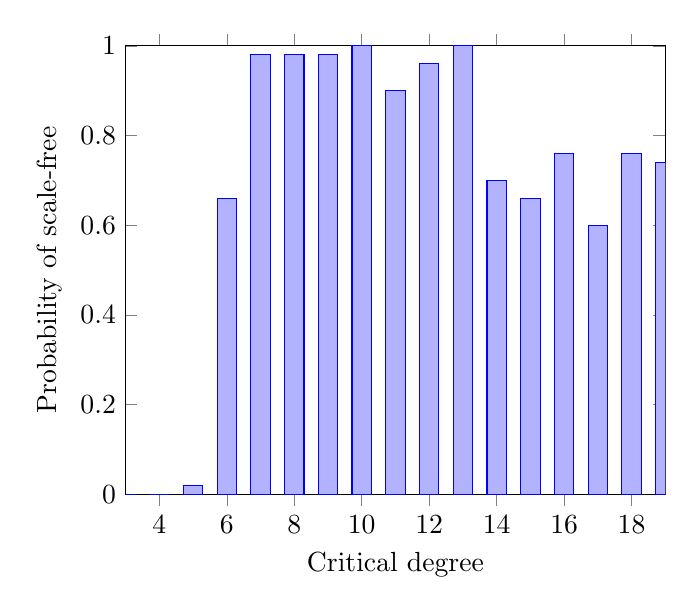
\begin{tikzpicture}
\begin{axis}[
x tick label style={
	/pgf/number format/1000 sep=},
	ylabel=Probability of scale-free,
	xlabel=Critical degree,
enlargelimits=0.0,
legend style={at={(0.5,-0.15)},
anchor=north,legend columns=-1},
ybar,
bar width=7pt,
]
\addplot
coordinates {
(3,0.0) (4,0.0) (5,0.02) (6,0.66) (7,0.98) 
(8,0.98) (9,0.98) (10,1.00) (11,0.90) (12,0.96)
 (13,1) (14,0.7) (15,0.66) 
(16,0.76) (17,0.60) (18,0.76) (19,0.74) };
\end{axis}
\end{tikzpicture}
\caption{\label{fig:PlotStarIsj} Shows the probability of the network ending up in a scale-free structure, given different critical degrees.}
\end{figure}
\subparagraph{Price of Anarchy.}
Another interesting thing is the average price of anarchy as function of the critical degree. The price of anarchy where calculated by taking the average total payoffs and dividing on the optimal payoff. The result can be seen in Figure \ref{fig:plotpriceofanarchy}. 

We see that the price of anarchy for the first critical degrees is 1, and then decreases until degree six, and at seven it increases again. This is because at degree one to five, the socially optimal structure is a clique, at degree six, a clique and a star, are almost equally good, and at degree seven and up a star-structure is the socially optimal outcome. 
In other words, when the cost is low, then a clique is the optimal structure, and when the cost is high a star is the optimal structure. 

This is further improves our findings, because now we have shown how an insurer can determine the resulting network formation by changing the cost, and also the formation that evolves also has a price of anarchy close to 1. 

\begin{figure}
\centering
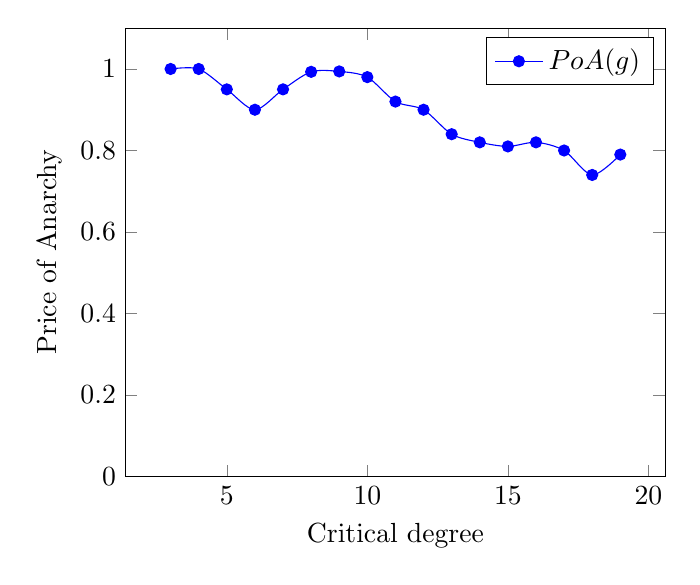
\begin{tikzpicture}
\begin{axis}[
	ylabel=Price of Anarchy,
	ymin=0.0,
	xlabel=Critical degree]
\addplot [smooth,mark=*,blue] plot coordinates {

(3,1) (4,1) (5,0.95) (6,0.9) (7,0.95) 
(8,0.993) (9,0.994) (10,0.98) (11,0.92) (12,0.90)
 (13,0.84) (14,0.82) (15,0.81) 
(16,0.82) (17,0.8) (18,0.74) (19,0.79) };
\addlegendentry{$PoA(g)$}
\end{axis}
\end{tikzpicture}
\caption{\label{fig:plotpriceofanarchy} Shows the price of anarchy as a function of critical degree}
\end{figure}

\subparagraph{Example structures from the simulation.}

\begin{figure}[h]
\centering
\begin{subfigure}{.9\textwidth}
  \centering
  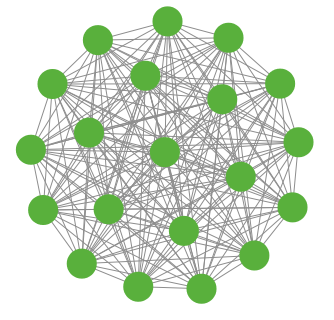
\includegraphics[width=0.7\linewidth]{../Figures/Clique-20-nodes.png}
  \caption{\label{fig:discountclique} A clique consisting of twenty nodes. }
\end{subfigure}
\quad
\begin{subfigure}{.9\textwidth}
  \centering
  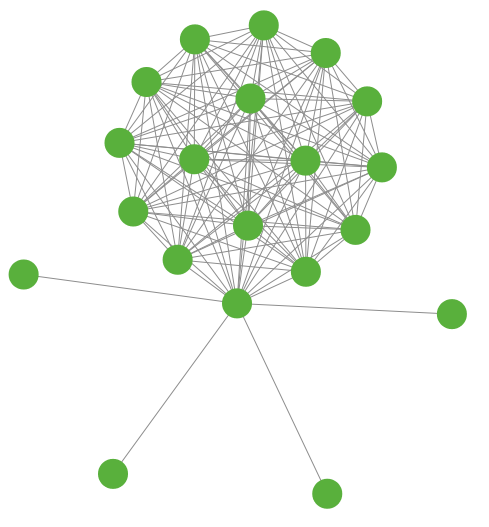
\includegraphics[width=0.7\linewidth]{../Figures/Clique-ish-20-nodes.png}
  \caption{\label{fig:discountbaloon} A network with high average node degree, but not a clique.}
\end{subfigure}
\caption{\label{fig:discounthighdegree} Two different outcomes of the simulations where the critical degree is low}
\end{figure}
In Figure \ref{fig:discounthighdegree} we see two of the many possible outcomes when the critical degree is achieved at a low node degree. As we see most of the nodes have reached the critical degree, and thus connected to every other node.
In Figure \ref{fig:star1} we see one example of a scalefree network, and the standard star network, both with twenty nodes and results from the simulations when the critical degree were set to a value above six. 
\begin{figure}[h]
\centering
\begin{subfigure}{.9\textwidth}
  \centering
 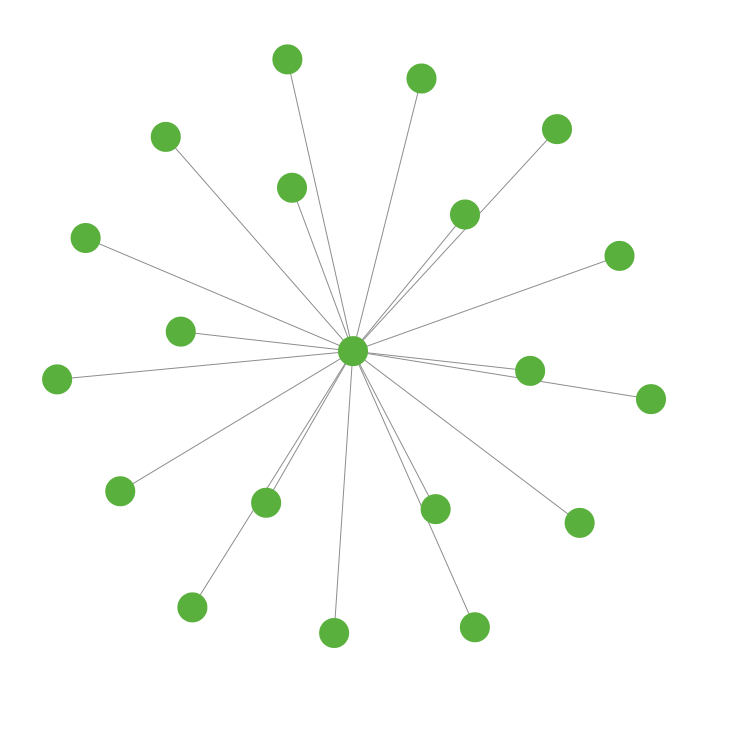
\includegraphics[width=0.7\linewidth]{../Figures/Star-20-nodes.png}
  \caption{\label{fig:star:a} A star consisting of twenty nodes}
\end{subfigure}
\quad
  
\begin{subfigure}{.9\textwidth}
  \centering
  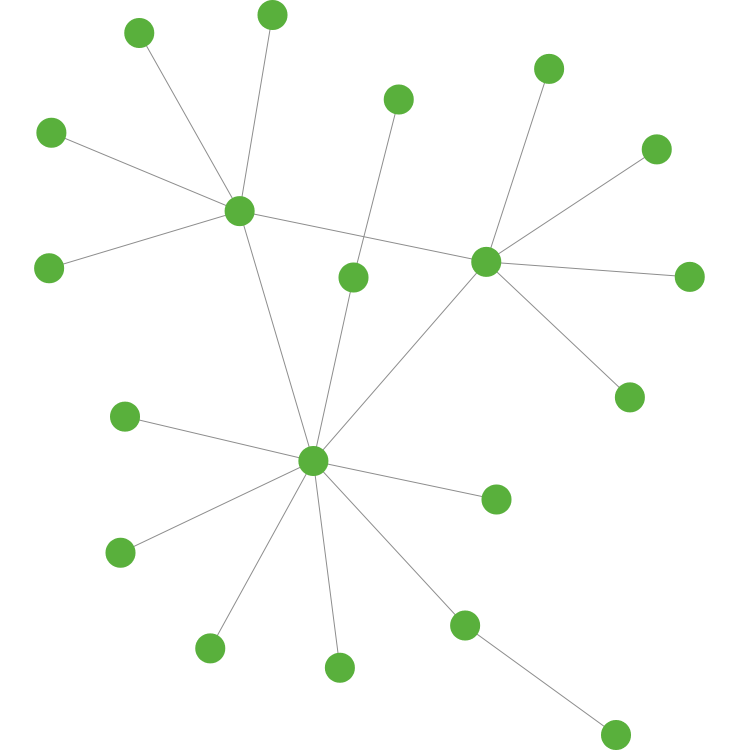
\includegraphics[width=0.7\linewidth]{../Figures/Scalefree-20-nodes.png}
  \caption{\label{fig:star:b} A scalefree network with twenty nodes, where three nodes account for most of the connectivity.}
\end{subfigure}
\caption{\label{fig:star1} Two different outcomes from running simulations with a high critical degree.}
\end{figure}






